\subsection{Parameter Settings}

In this section, we evaluate the practicality and optimality of various HTLP constructions based on the parameters $M,n,m,w$ of the auction or vote. 
% As discussed in~\Cref{sec:packing}, the size of the applied integer representations of ballots/bids increases linearly in certain parameters of the voting/auction schemes, e.g., the number of candidates. This limits the applicability of certain HTLP constructions instantiated in specific cryptographic groups, as we show next.  
Assuming the classic PNS packing, we require $(nw+1)^m\leq\vert\mathbb{G}\vert$ for voting and $M^n\leq\vert\mathbb{G}\vert$ for auctions, where $\mathbb{G}$ is the group in which the HTLP is instantiated.
We show the optimal HTLP construction for auctions and voting for various parameter settings in \Cref{fig:packed_feasibility} (with packing) and \Cref{fig:nopack_feasibility} (without packing). We use the security parameter $\secpar=80$ (see discussion in \Cref{sec:implementation}), which corresponds to a $1024$-bit modulus $N$ for exponential ElGamal and Paillier HTLPs and $3400$-bit discriminants for class group HTLPs. For the exponential ElGamal HTLP, we fixed the maximum ballot at $2^{80}$, which corresponds to $\approx 2^{40}$ brute-forcing work using Pollard's rho algorithm~\cite{Pollard78}.

\begin{figure}[tb!]
    \centering
    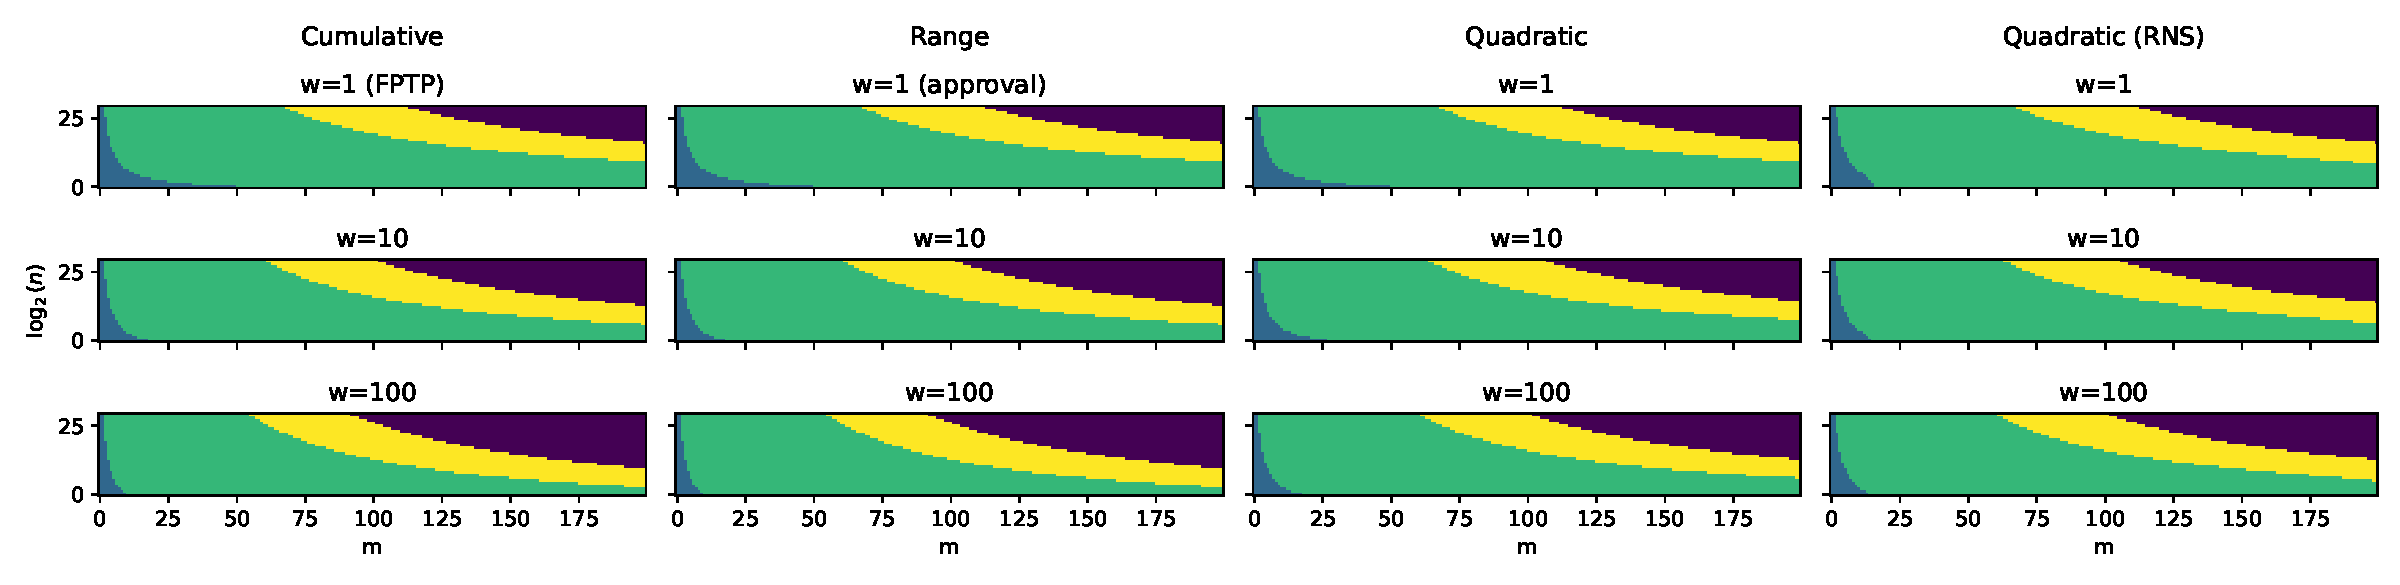
\includegraphics[width=\textwidth]{cicada/figs/params/pack_crq.pdf}
% \includegraphics[scale=0.56,trim={0.5cm 3cm 0.2cm 4.5cm},clip]
    \centering  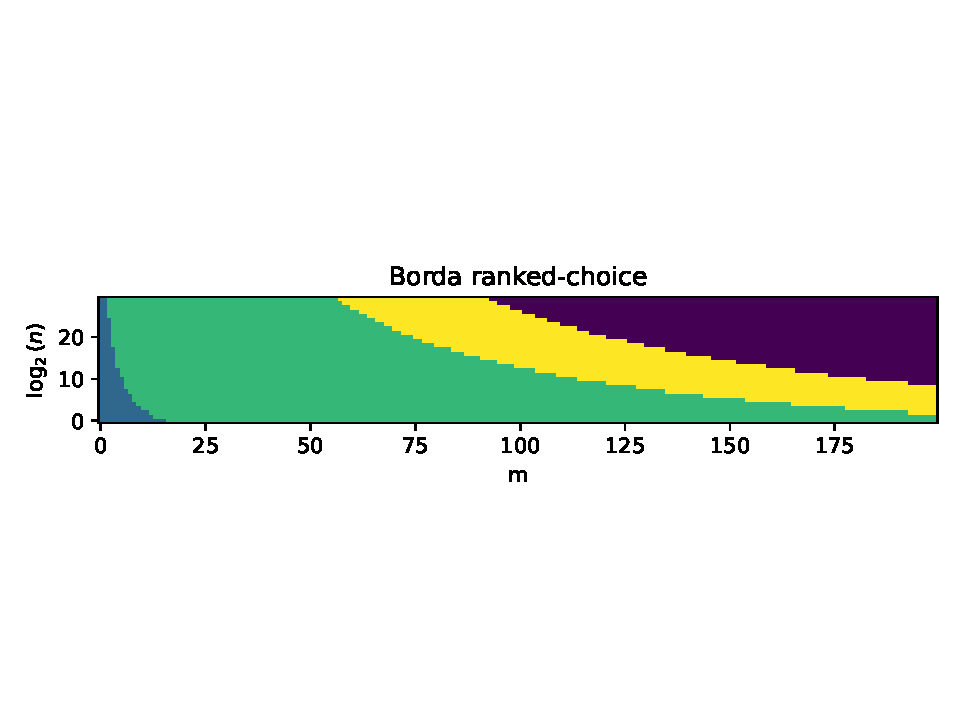
\includegraphics[width=0.45\textwidth,trim={0cm 3cm 0cm 4.5cm},clip]{cicada/figs/params/pack_borda.pdf}  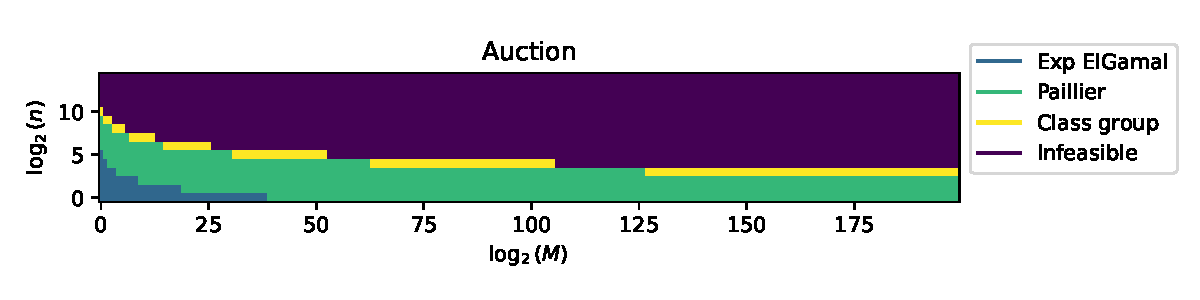
\includegraphics[width=0.5\textwidth,trim={0cm -1cm 0cm 4.5cm}]{cicada/figs/params/pack_auction.pdf}
    \caption{Most efficient HTLP construction for voting and auction using Cicada with maximal packing (using PNS except where indicated).}
    \label{fig:packed_feasibility}
\end{figure}

\begin{figure}[tb!]
    \centering
    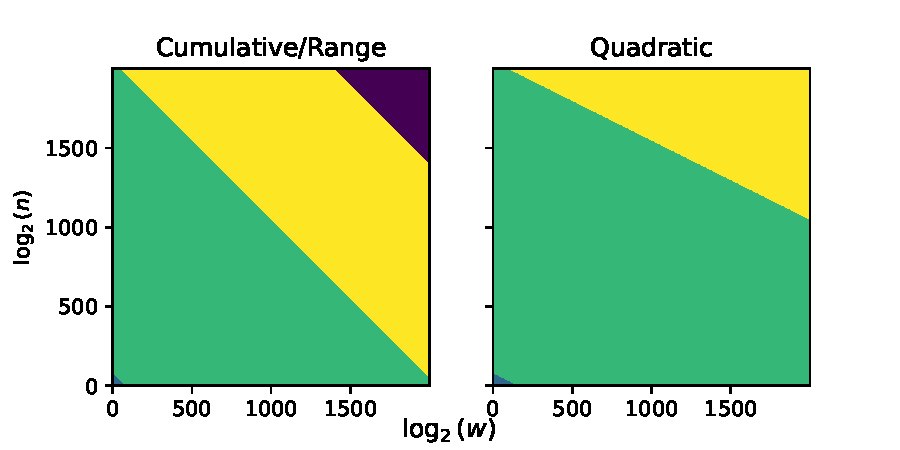
\includegraphics[width=0.49\textwidth,trim={0cm -0.5cm 0cm 0cm}]{cicada/figs/params/nopack_crq.pdf}
    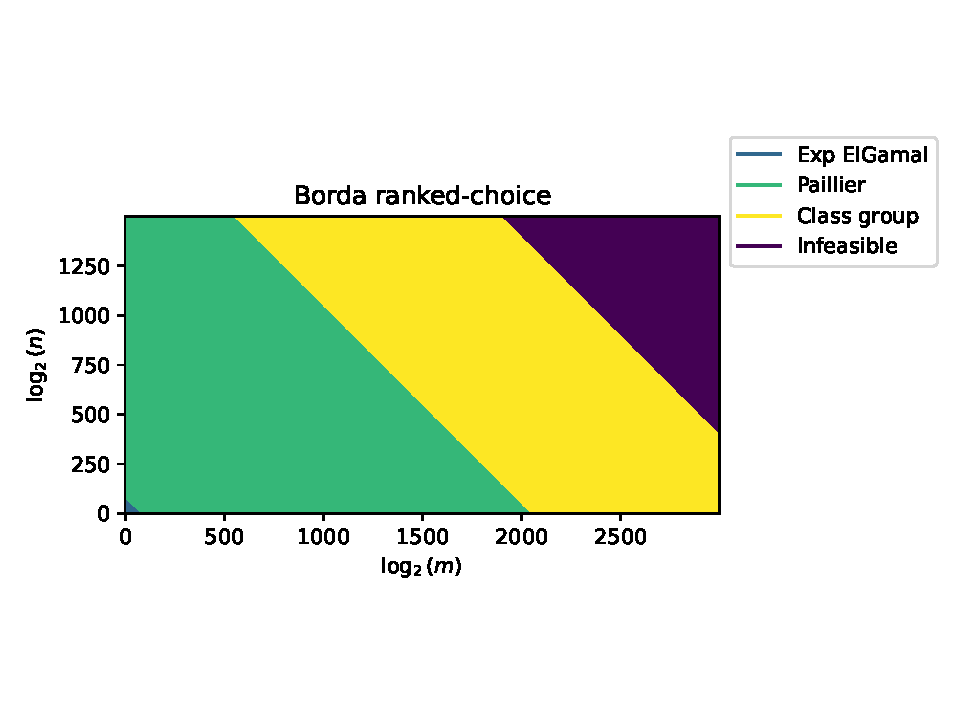
\includegraphics[width=0.49\textwidth,trim={2cm 2cm 0cm 2cm},clip]{cicada/figs/params/nopack_borda.pdf}
    \caption{Most efficient HTLP construction for voting schemes using Cicada without packing. For the sealed-bid auction, the bid bit-length directly determines the HTLP construction to use (exponential ElGamal up to 80 bits, then Paillier up to 2048, and class group up to 3400).}
    \label{fig:nopack_feasibility}
\end{figure}

\paragraph{Exponential ElGamal HTLP (\Cref{con:exp_elgamalHTLP})} 
This is the most efficient HTLP construction: for a given security parameter, it has the smallest required cryptographic groups and most efficient group operations. However, since the puzzle solution is encoded in the exponent, solving the puzzle requires brute-forcing a discrete logarithm. This limits the use of this construction to a small set of parameter settings: assuming the largest discrete logarithm an off-chain solver can be expected to brute-force has $\tau$ bits, we require $(nw+1)^m \leq 2^{2\tau}$.

\paragraph{Paillier HTLP (\Cref{con:paillierHTLP})} 
This is a slightly less efficient construction since the size of the HTLPs for a given security parameter is doubled due to working over $\bmod~N^2$ instead of $\bmod~N$. This increases both the required storage and the complexity of the group operation. On the other hand, due to its larger solution space, the Paillier HTLP supports much broader parameter settings for a given security parameter.

\paragraph{Class group HTLP} 
Class group offer the sole HTLP construction without a trusted setup~\cite{CCS:TCLM21}. This comes at the cost of the largest groups for a given security parameter. Class groups are not widely supported by major cryptographic libraries, and their costly group operation makes blockchain deployment difficult. We are unaware of any class group implementations for Ethereum smart contracts.

\paragraph{Impractical parameter settings} 
Accommodating very large settings of $n,\allowbreak w,m,M$ requires larger groups, leading to group operations and storage requirements which are intolerably inefficient for certain applications.